\section{Ideale Quantengase}
\subsection{Ideales Fermigas}

\begin{align}
    H &= \sum_j \epsilon_j  \hat n_j 
\end{align}
Freies Teilchen (Raum, Festkörper) 
\begin{align}
    \epsilon_{\vec k, \sigma} &= \frac{\hbar^2 \vec k^2}{2m^*} +\frac12 g^* \mu_B \sigma |\vec B| \\
\intertext{Großkanonische Zustandssumme}
    Z_\text{gk} &= Tr[e^{-\beta(\hat H - \mu \hat N)}] \\
\intertext{Kanonische Zustandssumme}
    Z_k &= \Tr[\e^{-\beta \hat H}]_{N = \text{const.}} \\
\intertext{Besetzungszahlbasis:}
    \Ket{n_1,n_2,...,n_j,...} \\
\text{Fermion:} \quad n_j  &= 0,1 \\
\text{Boson:} \quad n_j &= 0,1,2,...  \quad \in \mathbb{N}_0\\
    \hat n_j \Ket{n_1, ... n_j, ...} &= n_j \Ket{n_1, ....} \\
    N &= \sum_{j=1}^{\infty} n_j \qquad
    \hat N = \sum_{j=1}^{\infty} \hat n_j \qquad
    [\hat n_i, \hat n_j] = 0\\
    \hat F &= \e^{-\beta(\hat{H}-\mu \hat{N})} = \e^{-\beta \left(\sum_{j=1}^{\infty} (\epsilon_j - \mu) \hat{n}_j \right)} \\
    &= \prod_{j=1}^{\infty} \left( \e^{-\beta(\epsilon_j-\mu) \hat{n}_j} \right) = \prod_{j=1}^{\infty} F_j((\hat n)_j) \\
    \Tr[\hat F]_{\text{gk}}&= \Tr\left[\prod_{j=1}^\infty F_j(\hat n_j)\right]_{\text{gk}}\\
    &=\sum_{\{n_j=0,1\}} \Bra{n_1,n_2,...,n_j,...}\underbrace{\prod_{j=1}^\infty F_j(\hat n)\Ket{n_1,...,n_j,...}}_{\prod_{j=1}^\infty F_j(n_j)}\\
    &=\sum_{\{n_j=0,1\}} \prod_{j=1}^{\infty}F_j(n_j)\\
    &= \prod_{j=1}^\infty (F_j (0) + F_j (1))\\
    \Rightarrow Z_\text{gk} &= \prod_{j=1}^\infty \underbrace{(1+\e^{-\beta(\epsilon_j-\mu)})}_{Z_j} = \prod_{j=1}^\infty Z_j\\
    \Braket{\hat n_j} &= \frac1{Z_{\text{gk}}} \Tr[\e^{-\beta H -\mu\hat N} \hat n_j] = \frac{\cancel{\prod_{n \neq j}^{\infty} Z_n} (0 + \e{-\beta (\epsilon_j - \mu )})}{\cancel{\prod_{n=1}^\infty} \underarrow{Z_n}{Z_j}}
\end{align}
\begin{figure}[H]
  \centering
  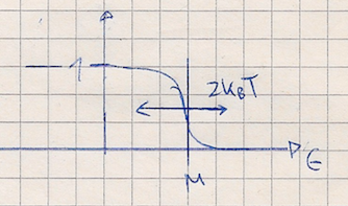
\includegraphics[width = \textwidth]{Zeichnungen/26.pdf}
  \caption{Energie.}
  %\label{fig:Bild}
\end{figure}
\begin{align}
    &= \frac{\e^{-\beta(\epsilon_j - \mu)}}{1+e^{-\beta(\epsilon_j - \mu)}} = \frac{1}{1 + e^{\beta(\epsilon_j - \mu)}+1} = \underarrow{f(\epsilon_j-\mu)}{\text{Fermi-Funktion}} 
\end{align}
\paragraph{Großkanonisches-Potential}
\begin{align}
    \Phi(T,\mu)=-\frac{1}{\beta}\ln Z_{\text{gk}}=-k_B T\sum_{j=1}^{\infty} \ln\left(1+\e^{-\beta(\epsilon_j-\mu)}\right)
\end{align}
\paragraph{Teilchenzahl}
\begin{align} 
    N &= -\pdif{\Phi}{\mu} = \frac{1}{\cancel{\beta}} \sum_{j=1}^{\infty} \underbrace{\frac1{1+\e^{-\beta(\epsilon_j - \mu)}} \cancel{\beta} \e^{-\beta (\epsilon_j - \mu)}}_{f(\epsilon_j - \mu)} \\
    N&=\sum_{j=1}^\infty \Braket{\hat n_j}=\sum_{j=1}^\infty f(\epsilon_j-\mu)
\end{align}
\paragraph{Innere Energie}
\begin{align}
    U = \Braket{\hat{H}} = \sum_{j=1}^{\infty} \epsilon_j f(\epsilon_j - \mu) = - \pdif{\Phi}{\beta}\biggr\rvert_{\beta \mu= \text{const.}}
\end{align}
\paragraph{Entropie}
\begin{align}
    S &= -\pdif{\Phi}{T} = \left(\pdif{\Phi}{\beta}\right) \left(\pdif{\beta}{T}\right) = k_\text{B} \beta^2 \pdif{\Phi}{\beta} \\  
    \pdif{\Phi}{\beta}&= \frac{1}{\beta^2} \ln Z_{\text{gk}}-\frac{1}{\beta} \sum_j \pdif{}{\beta} \ln Z_j\\
    &=\frac{1}{\beta^2} \ln Z_\text{gk}-\frac{1}{\beta^2} \sum_j \frac{1}{1+\e^{-\beta(\epsilon_j-\mu)}} \beta \left(-(\epsilon_j -\mu)\right) \e^{-\beta}\\
    &= \frac{1}{\beta^2} \ln Z_\text{gk} + \frac{1}{\beta^2} \sum_j \beta(\epsilon_j - \mu) f_j \\
    1-f_j &= 1- \frac1{\e^{\beta (\epsilon_j - \mu }+1} = \frac{\e^{\beta (\epsilon_j - \mu }}{\e^{\beta (\epsilon_j - \mu } + 1} = \frac1{Z_j}\\
    \ln(Z_j)&=-\ln(1-f_j)\\
    \beta(\epsilon_j-\mu) &= \ln(\underbrace{\e^{-\beta(\epsilon_j-\mu)}+1}_{\sfrac{1}{f_j}}-1)=\ln\left(\frac{1-f_j}{f_j}\right)=\ln(1-f_j)-\ln f_j\\
    S&=k_B\sum_{j=1}^\infty \ln(Z_j)+\beta(\epsilon_j-\mu) f_j\\
    &=k_B \sum_{j=1}^\infty \left(\left(-\ln(1-f_j)\right)+\left(\ln(1-f_j)-\ln f_j\right)f_j\right)\\
    &=-k_B\sum_{j=1}^\infty\left(\underbrace{f_j}_{P_j^1}\ln f_j +\underbrace{(1-f_j)}_{P_j^0}\ln(1-f_j)\right)\\
    S&= -k_B\sum_{j=1}^\infty \left( P_j^0 \ln P_j^0 + P_j^1 \ln P_j^0 \right) \checkmark
\end{align}

Dispersion eines freien Teilchens 
\begin{align}
    \epsilon_{\vec k} &= \frac{\hbar^2 k^2}{2m}\\
    \Rightarrow U&=\sum_j \epsilon_j f(\epsilon-\mu)=\sum_{\vec k \sigma} \epsilon_{\vec k \sigma} \underarrow{f}{\text{Fermifunktion hängt nur von der Energie ab!}}(\epsilon_{\vec k \sigma}-\mu) \\
\intertext{Zustandsdichte:}
    \rho_\sigma &= \frac1V \sum_{\vec k} \delta(\epsilon-\epsilon_{\vec k, \sigma}) \\
    \Rightarrow \Aboxed{U &= \sum_\sigma V \int_{-\infty}^{\infty} \symup{d} \epsilon \rho_\sigma (\epsilon) f(\epsilon - \mu)}\\
    N &= \sum_j f(\epsilon_j - N ) = \underarrow{2V}{\sum_\sigma} \int_{-\infty}^{\infty} \dif \epsilon \ \rho(\epsilon) f(\epsilon-\mu)\epsilon \\
    \Aboxed{n &= \frac{1}{v}=2 \int_{-\infty}^{\infty} \dif \epsilon \rho(\epsilon) f(\epsilon-\mu)} \\ &\text{Imp\emph{lizite?} Gleichung für $\mu$ bei kanonischer Rechnung} \\
    n &= \frac1v = \frac NV
\end{align}
\begin{figure}[H]
  \centering
  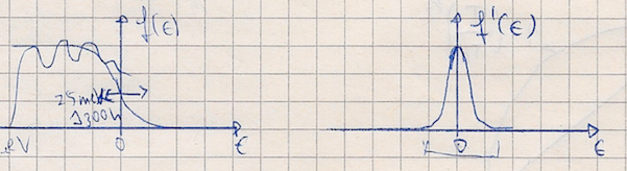
\includegraphics[width = \textwidth]{Zeichnungen/27.pdf}
  \caption{.}
  %\label{fig:Bild}
\end{figure}
\begin{align}
\intertext{Integrale vom Typ:}
    \int_{-\infty}^\infty \dif \epsilon f(\epsilon-\mu) I(\epsilon) &= \underbrace{\cancel{f(\epsilon)k(\epsilon)\biggr\rvert_{-\infty}^\infty}}_{=0} + \int_{-\infty}^\infty \dif \epsilon \left(-\pdif{f}{\epsilon}\right) K(\epsilon)\\
    K(\epsilon) &= \int_{-\infty}^{\epsilon} \dif \epsilon' I(\epsilon')\\
    -\pdif{f}{\epsilon} &=-\pdif{}{\epsilon}\left(\frac{1}{\e^{-\beta(\epsilon-\mu)}+1}\right) \\
    &=\frac{1}{\e^{-\beta(\epsilon-\mu)}+1} \frac{1}{\e^{-\beta \epsilon-\mu)}+1} \beta \e^{\beta(\epsilon-\mu)}\\
    &=\beta f(\epsilon -\mu)f(-(\epsilon-\mu))
\end{align}

\paragraph{Taylor-Entwicklung}
\begin{align}
    K(\epsilon)&=K(\mu)+\sum_{n=1}^{\infty} \frac{1}{n!}(\epsilon-\mu)^n \frac{\dif^n K(\epsilon)}{\dif \epsilon^n}\biggr\rvert_{\epsilon=\mu} \\
    \Aboxed{\int_{-\infty}^{\infty} \dif \epsilon f(\epsilon - \mu) I(\epsilon) &= \int_{-\infty}^{\mu} \dif \epsilon I(\epsilon) + \sum_{n=1}^{\infty} \frac{1}{n!} \frac{\dif^{n-1}I(\epsilon)}{\dif\epsilon^{n-1}}\biggr\rvert_{\epsilon = \mu} \underbrace{\int_{-\infty}^\infty \dif \epsilon \left(-\pdif{f}{\epsilon} \right) (\epsilon - \mu)^\mu}_{=0 \text{ für n ungerade}}}
    \intertext{Sommerfeld-Entwicklung}
\end{align}

Zustandsdichte
\begin{align}
    \rho(\epsilon) &= \frac{1}{v}\sum_{\vec k} \delta(\epsilon-\epsilon_{\vec k \epsilon})  \qquad \quad \text{z.B.} \epsilon_{\vec k}=\frac{\hbar^2 k}{2 m}\\
    %\int_{-\infty}^\infty \dif \epsilon f(\epsilon-\mu)I(\epsilon)=\int_{-\infty}^\mu \dif \epsilon I(\epsilon)+\sum_{n=1}^\infty \frac{1}{n!}
    %\frac{\dif^{n-1}I(\epsilon)}{\dif\epsilon^{n-1}}\biggr\rvert_{\epsilon = \mu} \underbrace{\int_{-\infty}^\infty \dif \epsilon \left(-\pdif{f}{\epsilon} \right) (\epsilon - \mu)^\mu}_{=0 \text{für n ungerade}}
    \int_{-\infty}^\infty (\epsilon - \mu)^{2n} \left(-\pdif{f}{\epsilon}\right) &= \underbrace{\beta \int_{-\infty}^\infty \dif \epsilon}_{\dif x}(\beta(\epsilon - \mu))^{2n} \frac{\e^{\beta (\epsilon-\mu)}}{(\e^{\beta (\epsilon-\mu)}+1)^2} \frac{1}{\beta^{2n}} \\
    &= (k_B T )^{2n}  \int_{-\infty}^\infty \dif x x^{2n} \frac{\e^{x}}{(\e^{x}-1)^2} = (k_B T)^{2n} A_{2n}\\
    f(\epsilon) = \frac1{\e^{\beta \epsilon}+1} \qquad x &= \beta(\epsilon - \mu) \qquad \dif x = \beta \dif \epsilon 
\end{align}
%
\begin{figure}[H]
  \centering
  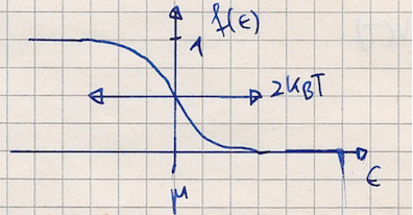
\includegraphics[width = \textwidth]{Zeichnungen/28.pdf}
  \caption{.}
  %\label{fig:Bild}
\end{figure}
%
\paragraph{$\Rightarrow$ Riemannsche $\zeta$-Funktion} 
\begin{align}
    \tdif{}{\lambda} \left(\frac{1}{\e^{\lambda x}+1}\right) &= - \frac{x \e ^{\lambda x}}{(\e^{\lambda x} +1)^2} \\
    A_{l = 2n} &= \int_{-\infty}^{\infty} \dif x x^l \frac{\e^x}{\left(\e^x + 1 \right)^2} = -2 \tdif{}{\lambda} \underbrace{\left[ \int_{-\infty}^{\infty} \dif x x^{l-1} \frac1{\e^{\lambda x} + 1} \right]}_{u = \lambda x \quad \dif u = \lambda \dif x}\\
    &=-2\tdif{}{\lambda}\left[\frac{1}{x^l}\int_0^\infty \dif u \frac{u^{l-1}}{\e^u + 1}\right]
    = 2l \int_{0}^\infty \dif U \frac{U^{l-1}}{\e^{U}+1}
\end{align}

\paragraph{Riemannsche $\zeta$-Funktion: Integraldarstellung}
\begin{align}
    \zeta (l) &= \frac1{(1-2^{l-1})\Gamma(l)} \int_0^\infty \dif U \frac{U^{l-1}}{\e^U +1} & \\
    A_{l=2n}&=2\underbrace{(2n)\underbrace{\Gamma(2n)}_{(2n-1)!}}_{(2n)!} \left(1-2^{1-2n}\right)\zeta(2n) & \Rightarrow A_0&=2(1-2^1)\underarrow{\zeta(0)}{-\frac12}=1\\
    &&   A_2&=2 2!(1-2^{1-2})\underarrow{\zeta(2)}{\frac{\pi^2}{6}}=\frac{\pi^2}{3}\\
\end{align}
\begin{align}
    I(\epsilon) &= \rho(\epsilon) \\
    n &= \frac1v = \underarrow{2}{\text{Spin}}\left[\int_{- \infty}^\mu \dif \epsilon \rho (\epsilon) + \frac{1}{2!} \rho' (\mu) (k_B T)^2 \frac{\pi^2}{3} + \mathcal O((k_B T)^4)\right]  \label{eqn:zeile117}\\
    U&=\frac{U}{V}=2\int_{-\infty}^\mu \dif \epsilon \ \epsilon \rho(\epsilon) +\tdif{}{\epsilon}\biggr\lvert_{\epsilon=\mu} (k_B T)^2 \frac{\pi^2}{3}+... \\
\intertext{Energiedichte $\quad \Phi(\epsilon) = \rho(\epsilon) \epsilon$}
\end{align}
\begin{align}
    U &= 2 \int_{-\infty}^{\infty} \dif \epsilon \ \epsilon \rho(\epsilon) + [\rho(\mu) + \mu \rho'(\mu)] (k_\text{B} T)^2 \frac{\pi^2}{3} + ... \label{eqn:zeile121}\\
    \eqref{eqn:zeile121}  \stackrel{T \to 0}{\rightarrow} \quad U_0 &= 2 \int_{-\infty}^{\mu_0} \dif \epsilon\ \epsilon \rho(\epsilon)\\
    \eqref{eqn:zeile117}  \stackrel{T \to 0}{\rightarrow}  \quad \frac1v &= 2 \int_{-\infty}^{\mu_0} \dif \epsilon \rho(\epsilon)\\
    \eqref{eqn:zeile117}-\eqref{eqn:zeile117} \text{bei $T=0$}:  0&=\left[\int_{\mu(0)}^{\mu(T)}\dif \epsilon \rho(\epsilon) +\frac{\pi^2}{6}\rho'(\mu)(k_B T)^2 +...\right]\\
    &\Rightarrow \mu(T)-\mu_0 \approx (k_B T)^2\\
    0 &\approx \rho(\mu_0)[\mu(T)-\mu_0]+\frac{\pi^2}{6}\rho'(\mu_0)(k_B T)^2+...\\
    \Aboxed{\mu(T) &= \mu_0 - \frac{\pi^2}{6} \frac{\rho'(\mu)}{\rho(\mu)} (k_B T)^2}
\end{align}
\begin{figure}[H]
  \centering
  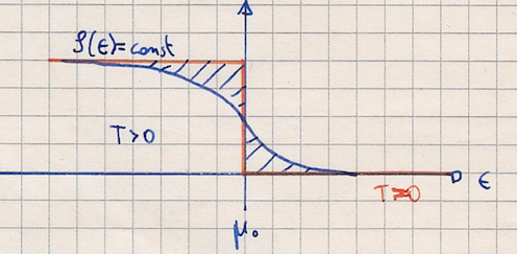
\includegraphics[width = \textwidth]{Zeichnungen/29.pdf}
  \caption{Übergang zur Sprungfunktion.}
  %\label{fig:Bild}
\end{figure}
\begin{align}
    \epsilon_k&=\frac{\hbar^2 k^2}{2 m} \qquad 3D:  \quad \rho \approx \sqrt{\epsilon} \quad \rho'(\mu)>0 
\end{align}
\begin{figure}[H]
  \centering
  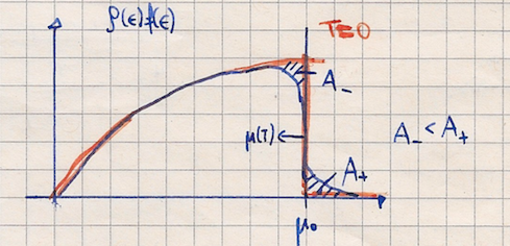
\includegraphics[width = \textwidth]{Zeichnungen/30.pdf}
  \caption{.}
  %\label{fig:Bild}
\end{figure}
\begin{align}
    U(T)-\frac{U(T=0)}{V} &= 2\left[\underarrow{(\mu(T)-\mu_0)}{\cancel{-\frac{\pi^2}{6}\frac{\rho'(\mu)}{\rho(\mu)}(k_B T)^2}}\mu_0\rho(\mu_0))+\frac{\pi^2}{6} (\rho(\mu_0)+\cancel{\mu_0 \rho'(\mu_0)})(k_B T)^2+...\right] \\
    &= \frac{\pi^2}{3} \rho(\mu_0) (k_B T)^2 
\end{align}

\paragraph{Spezifische Wärme}

\begin{align}
    C_V &= \pdif{U}{T}[V = \text{const.}] = V \pdif{}{T} [U(T)- U (0)] = 2V \frac{\pi^2}{3} \rho(\mu_0) k_B^2 T = \gamma T\\
\intertext{Gamma-Koeffizient: $\gamma = 2 U_B^2 \rho(\mu_0)\frac{\pi^2}{3}V$}
    C_v &\propto T \quad \text{und verschwindet für $T \to 0$}\\
    \sum_{\vec k} \underarrow{I(\epsilon_{\vec k})}{\delta(\epsilon-\epsilon_k) \epsilon=\frac{\hbar^2}{2m}k^2}&=\frac{V}{(2\pi)^d} \int \dif^d k \quad \quad \int\dif^d k=\int_0^\infty \dif k k^{d-1} O_d\\
    \rho(\epsilon) &= 
    \begin{cases}
    a\frac{1}{\sqrt{\epsilon}} &d=1\\
    a   &d=2\\
    a\sqrt{\epsilon}  &d=3 
    \end{cases} \qquad = a_x\epsilon^x
\end{align}
\begin{align}
    \Psi(T, N, V) &= - \frac1\beta \ln(Z_\text{gk}) = - 2 k_B T V \int_{-\infty}^{\infty} \dif \epsilon \rho(\epsilon) \ln(1 + \e^{-\beta(\epsilon-\mu)})\\
    N &= \sum_{??G} f(\epsilon_k - \mu) = 2 V \int_{-\infty}^\infty \dif \epsilon f(\epsilon-\mu) \rho(\epsilon)\\
    \int\dif\epsilon\rho(\epsilon)&=a \int \dif \epsilon \epsilon^x =\frac{a}{1+x}\epsilon^{1+x}=\frac{\epsilon}{1+x}\rho(\epsilon)
\intertext{Druck: (Zustandsgleichung)}
    p&=-\pdif{\Phi}{V}=2 k_B T \int_{-\infty}^\infty \dif \epsilon \rho(\epsilon) \ln(1+\e^{-\beta(\epsilon-\mu)}) \\
    &=2k_B T \left[\frac{\epsilon}{1+x}\rho(\epsilon) \ln(1+\e^{-\beta(\epsilon-\mu)})\right]_{-\infty}^\infty \\ 
    &\quad -\frac{1}{1+\epsilon}\int_{-\infty}^\infty \dif \epsilon \epsilon \rho(\epsilon) \underbrace{\frac{\beta \e^{-\beta(\epsilon-\mu)}}{1+\e^{-\beta(\epsilon-\mu)}}}_{-\beta f(\epsilon-\mu)}\\
    p &= \frac1{1+x} \underbrace{2 \int_{-\infty}^{\infty} \dif \epsilon \rho(\epsilon) \epsilon f(\epsilon - \mu)}_{\frac{U}{V}}\\
    \Rightarrow \Aboxed{pV &= \frac1{1+x}}\\
    \text{3D: } x &= \frac12 \\
    pV & =\frac32 U\\
    \intertext{ideales Gas: $U = \frac32 N k_B T$}
\end{align}

\paragraph{Grundzustand}

\begin{align}
    N &= \underarrow{2}{\text{Spin}} \frac{V}{\underbrace{(2 \pi)^3}_{d = 3}} \frac{4 \pi}{3} k_F^3\\
    k_F^2&=\left(\frac{3N\pi^2}{V}^{\frac23}\right)\\
    \Rightarrow \underarrow{\epsilon_F}{\text{Fermienergie}}&=\frac{\hbar^2}{2m}\left(\frac{3N\pi^2}{V}\right)^{\frac23}
\end{align}

\subsubsection{Klassischer Grenzfall}

\begin{align}
    \text{bisher: } T &\to 0 (\beta \to \infty)\\
    \text{jetzt: } T &\to \infty (\beta \to 0)\\
\intertext{Frage: Geht das Fermigas in das klassische ideale Gas über?}
    \text{Beispiel: } \epsilon_{\vec k} &= \frac{\hbar^2 k^2}{2m} \qquad 3D\\
    \Phi(T,\mu,V) &= - \frac{1}{\beta} \ln(Z_\text{gk}) = - k_\text{B} T \frac{2 V}{(2 \pi)^3} \int \dif^3k \ln \left( 1 + z \e^{-\beta \frac{\hbar^2 k^2}{2m}}  \right)\\
    z&=\e^{\beta \mu} \qquad \text{Fugazität} \\
    x &= k \sqrt{\frac{\beta \hbar^2}{2m}}; \quad \dif x = \hbar \sqrt{\frac{\beta}{2m}} \dif k \\ 
    \Phi &= - k_\text{B} T \frac{2 V}{(2 \pi)^3} \left(\sqrt{\frac{2m}{\beta \hbar^2}}\right)^3 4 \pi \int_0^\infty \dif x\ x^2 \ln(1 + z \e^{-x^2})\\
\intertext{Thermische de-Broglie-Wellenlänge:}
    \lambda_T(T) &= \frac{2 \pi \hbar}{\sqrt{2 \pi m k_\text{B}}} = \sqrt{\frac{2\pi \beta \hbar^2}{m}} \\
    \Phi&=-k_\text{B} \frac8{\sqrt{\pi}}\frac{V}{\lambda_T^3}
    \int_0^\infty \dif x\ x^2 \ln(1+\underbrace{z\e^{-x^2}}_{y})
\intertext{Taylorreihe:}
    \ln(1+y) &= \sum_{n=1}^{\infty} (-1)^{n+1} \frac{y^k}{k} \quad |y| \leq 1 \\
    \int_0^\infty \dif x \ln \left( 1 + z e^{-x^2} \right) x^2
    & =\sum_{n=1}^\infty (-1)^{k+1}\frac{z^n}{n} \int_0^\infty \dif x \underbrace{x^2 e^{-nx^2}}_{-\tdif{}{n} \e^{nx^2}} \\
    &= \sum_{n=1}{\infty} (-1)^{n+1} \frac{z^n}{n} (- \tdif{}{n} \frac{\sqrt{\pi}}{2} \underarrow{n^{-\frac12}}{-\frac12 n^{-\frac32}}) \\
    &= \frac{\sqrt{\pi}}{4} \sum_{n=1}^\infty (-1)^{n+1} \frac{z^n}{n^{\frac{5}{2}}} = \frac{\sqrt{\pi}}{4} f_{\frac{5}{2}}(z) \\
    f_{\frac32}(z)&=z\tdif{}{z} f_{\frac52}(z)=z\sum_{n=1}^\infty (-1)^{n+1}\frac{\cancel{n}z^{n-1}}{n^{\cancel{\frac52}\frac32}} =\sum_{n=1}^\infty (-1)^{n+1} \frac{z^{n}}{n^{\frac32}} \\
    \Rightarrow \Phi(T, \mu, V) &= - k_B T \frac{2V}{\lambda_T^3 f_{\frac52(z)}}\\
\intertext{Zustandsgleichung:}
    p &= -\pdif{\Phi}{V} = k_\text{B} T \frac{1}{{\lambda_T}^3} f_{\frac{5}{2}}(z) \\
    N &= z \tdif{}{z} \ln(Z_{\text{gk}}) = 2 V z  \tdif{}{z} \frac1{\lambda^3} f_\frac52 (z)\\
    \Aboxed{N &= \frac{2V}{\lambda_T^3} f_\frac{5}{2}} \label{eqn:zeile205} \\
    \text{Für } \beta \to 0 (t \to \infty) \quad &\Rightarrow \lambda_T \to 0 \quad \Rightarrow \frac1{\lambda_T} \to \infty \\
    &\text{Aus} \stackrel{\eqref{eqn:zeile205}}{\rightarrow} f_{\frac52}(z)\rightarrow 0 , z \rightarrow 0\\
    z\rightarrow 0: f_{\frac{3}{2}(\frac{5}{2})}(z)&\approx z-\frac{z^2}{2^{\frac{3}{2}(\frac{5}{2})}}\\
\intertext{Aus \eqref{eqn:zeile205}}
    \text{0. Näherung:} z_0 &= \frac{n \lambda_T^3}{2} \quad ; n= \frac NV \\
    \frac{n \lambda_T}{2} &= f_\frac32 (z) = z_0 = z_1 \left(1 - \frac{z_0}{2^\frac32}\right)\\ 
    z_1 &\approx \frac{z_0}{1-\frac{z_0}{2^\frac{3}{2}}} \approx z_0\left(1+\frac{z_0}{2^{\frac{3}{2}}}\right) \\
    pV &= \frac{k_\text{B}T}{\lambda_T^3} \frac{2V}{N} \left[ \underarrow{z}{z_1} - \underarrow{z^2}{z_0^2}\frac{1}{2^{\frac{5}{2}}} + \mathcal O(z^3)\right]\cdot N\\
    &= k_B T N \cancel{\frac1z_0} \cancel{z_0} \left[1+ \frac{z_0^2}{2^\frac32} -\frac{z_0}{2^\frac52} + O(z_0^2)\right]\\ 
    pV&=k_\text{B}TN\left[\underarrow{1}{\text{Ideales Gas}\hspace{2cm}}+\underarrow{\frac{n \lambda_T^3}{2}\frac{1}{2^{\frac52}}}{\hspace{2cm}\text{Quantenkorrekturen}}+O(z_0^2)\right]
\end{align}
\subsection{Das ideale Bose-Gas}
\begin{align}
    H&=\sum_{\vec k} \epsilon_{\vec k} \hat n_k=\sum_{\vec k}  \epsilon_{\vec n}  b^\dagger_k b_k \\
    [b_{\vec k}, b_{\vec k'}^\dagger] &= \delta_{\vec k, \vec k'} \quad ; \epsilon_k=\frac{\hbar^2 k^2}{2m}\\
    \Tr\left[\prod_{\vec k} F_k(\hat n_k)\right]_{\text{Fock-Raum}} &= \prod_K \Tr\left[F_{\vec k}(\hat n_k)\right]\\
    Z_{\vec k} &= \Tr \left[ \e^{-\beta(\epsilon_{\vec k} - \mu)\hat n_k} \right] = \sum_{n=0}^\infty[\e^{\beta(\epsilon_k-\mu)}]^k = \frac1{1-e^{-\beta (\epsilon_k - \mu)}} \\
    \Braket{\hat n_k} \frac{1}{z_k}\Tr[\hat n_k \e^{-\beta(\epsilon_k-\mu)\hat n_k}]
    &= \frac{\e^{-\beta (\epsilon_{\vec k}- \mu)}}{1- \e^{-\beta (\epsilon_{\vec k}- \mu)}} = \frac{1}{\e^{-\beta (\epsilon_{\vec k}- \mu)}-1} = \underarrow{g}{\text{Bose-Funktion}}(\epsilon_{\vec k} - \mu)\\
    \Braket{n}&=-\frac{1}{\beta}\pdif{\ln(z)}{\epsilon}
\end{align}
\begin{align}
\intertext{Thermodynamisches Potential}
    \Phi(T, \mu, N) &= k_\text{B} T \sum_k \ln(1-\e^{-\beta \epsilon_k -\mu}) \\
    N & = \sum_{\vec k} g(\epsilon_{\vec k} - \mu) \qquad S = \pdif{\Phi}{T}
\end{align}
\begin{figure}[H]
  \centering
  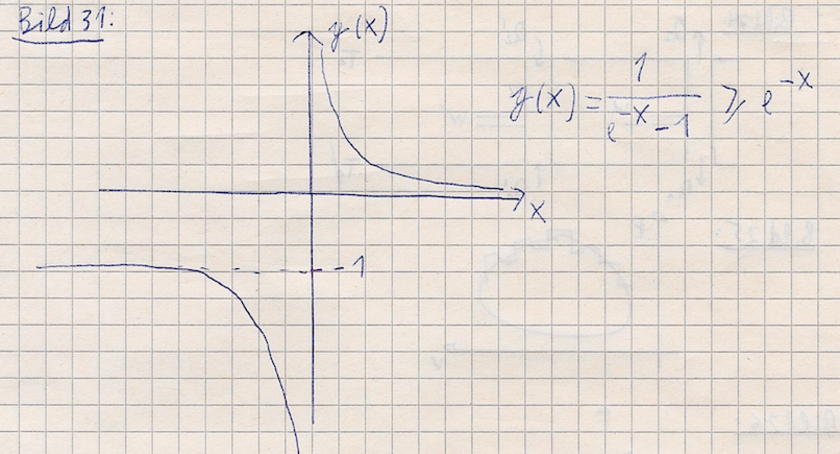
\includegraphics[width = \textwidth]{Zeichnungen/31.pdf}
  \caption{.}
  %\label{fig:Bild}
\end{figure}
\begin{align}
\intertext{Bose-Funktion singulär bei $\beta x \to 0$}
    \e^{\beta x} \approx 1 + \beta x \\
    \Rightarrow g(x) &= \frac{1}{e^{\beta x} -1} \approx \frac{1}{1+\beta x -1} \approx \frac{1}{\beta x} \\ 
    g(x) &< 0 \quad \text{für} \quad x < 0 \\ 
    g(x) &= \frac{1 - \e^{\beta x} + \e^{\beta x}}{\e^{\beta x} - 1} = -1 + \frac{\e^{\beta x}}{\e^{\beta x} -1} \to -1 - \e^{\beta x} \quad \text{für} \quad \beta x \to - \infty \\
    \text{Da }
    &\begin{drcases*}
     n_k= \Braket{\hat n_k} & $\geq 0$\\
     \text{und} \ \epsilon &$\geq 0$
    \end{drcases*} %hoffentlich klappt das 
    \Rightarrow \mu \leq 0\\
    N &= V \int_0^\infty \dif \epsilon \underarrow{\rho(\epsilon)}{a_q \epsilon^{\frac{d-2}{2}}} g(\epsilon-\mu)\geq V a \int_{0}^{\infty} \dif \epsilon \ \epsilon^{\frac{d}{2} - 1} \underbrace{\e^{-\beta(\epsilon - \mu)}}_{\e^{\beta \mu}} \e^{-\beta \epsilon} \frac{\beta^{\frac{d}{2}-1}}{\beta^{\frac{d}{2}-1}} \frac{\beta}{\beta} \\
    &= Va \beta^{-\frac{d}{2}}\e^{\beta\mu}\underbrace{\int_0^\infty \dif x \e^{-x} x^{\frac{d}{2}-1}}_{A} \\
    \Rightarrow - \beta \mu &\approx \ln(\beta^{-\frac{d}{2}}) \\
    \Rightarrow \mu &\approx -T \ln(T) \\
    \text{Für} \to 0  \quad \mu(T) &\to 0^- \\
    T \to 0 &\quad \epsilon_k = 0 \\
    N&=\underarrow{g_0}{\text{Grundzustand makroskopisch besetzt}}=\frac1{\e^{\beta(\epsilon-\mu)}-1} = \frac{z}{z-1} \quad z=\e^{\beta \mu} \\
    \Rightarrow \mu(T) &\approx-bk_\text{B}T\\
    \Rightarrow N &\approx \frac1{\e^b -1} \\
    b &\approx \ln \left( 1 + \frac1{N} \right) \approx \frac1{N} \\
    M_k&=\sum_{\vec k}(\epsilon_{\vec k}^k g(\epsilon-\mu)=g_0 \delta_{k,0}+\sum_{\vec k, \epsilon_{\vec k}g_0} (\epsilon_{\vec k})^k g(\epsilon-\mu)  
\end{align}
\paragraph{Ideales Bose-Gas}
\begin{align}
    %g(x)&=\frac{1}{\e^{\beta x-\mu}-1} \stackrel{\epsilon = 0}{=} \frac{1}{\frac{1}{z} -1} = \frac{z}{1-z} \\
\end{align}
\begin{itemize}
      \item $\lim{x\to0^+}g(x)\to \infty$
      \item Grundzustandsbesetzung kann makroskopisch werden $g(\epsilon)\propto O(N)$
      \item $g(\epsilon)=\Braket{n_\epsilon}\geq 0 \rightarrow$ schränkt die Wertemenge von $M$ ein
\end{itemize}
\begin{align}
    M_n &= \sum_{\vec k} (\epsilon_{\vec k})^n g(\epsilon_{\vec k})
    \underarrow{=}{\epsilon=0: \text{ Grundzustandsenergie}}
    g_0\delta_{n,0}+\sum_{\vec k,\epsilon_{\vec k}g_0} (\epsilon_{\vec k})^n g_k(\epsilon_{\vec k}-\mu)\\
    \Aboxed{N=M_0,&\quad U=M_1} \\
    \vec p&=\hbar \vec k\\
    M_n&= g_0\delta_{n,0}+\frac{V}{(2\pi\hbar)^d} O_d \int_0^\infty \dif p
    p^{d-1} \left(\frac{p^2}{2M}\right)^n \frac{1}{\frac{1}{z}\e^{\beta\frac{p^2}{2M}}-1 }\\
    O_d &= \frac{2\pi^{\frac{d}{2}}}{\Gamma(\frac{d}{2})} \quad \text{Oberfläche der $d$-dimensionalen Einheitskugel}\\
    &=\underbrace{...}_\text{Nebenrechnung}=g_0\delta_{n,0} + \frac{V}{{\lambda_T}^d}(k_\text{B}T)^n C_n^d g_{n+\frac{d}{2}}(z) \\
    g_n(z) &= \sum_{l=1}^\infty \frac{z^l}{l^k} = \Li_n(z) \qquad \text{Polylogarithmus}\\
    \text{Li}_1(z)&=-\ln(1-z)\\
    C_n^d&=\prod_{i=1}^n (n-i+\frac{d}{2}) \quad C_0^d =1\\
    \Rightarrow  \Aboxed{N &= \frac{z}{1-z} + \frac{V}{\lambda_T^d} g_{\frac d2}(z)}\\
    \Aboxed{U &= \frac{v}{{\lambda_T}^d} \cdot  \frac{d}{2} g_{1+\frac{d}{2}}(z) \kB T}  \\
\intertext{ Implizite Gleichung für M (oder $z=\e^{\beta M}$)}
\intertext{Zustandsgleichung}
    p&=-\pdif{\Phi(T,\mu,V)}{V} \quad \text{mit} \quad \Phi = -\frac{1}{\beta} \ln(Z_{\text{gk}}) = -\kB T \sum_k \ln(Z_k)\\
    \frac{p V}{\kB T} &= \frac{V}{(2 \pi \hbar)^d} O_d \int_0^\infty \dif p p^{d-1} \ln\left(1- z \e^{-\beta \frac{p^2}{2m}}\right) = \frac{V}{\lambda_T^d} g_{1+\frac{d}{2}} (z)\\
    \ln(1-z \e^{-\frac{\beta p^2}{2m}})&=-\sum_{l=1}^\infty \frac{1}{l}\left(z\e^{-\frac{\beta p^2}{2m}}\right)^l\\
    \Aboxed{pV &= \frac{2}{d}U} \qquad \text{identisch zum Fermigas} \\
    \lambda_T(T)&=\frac{2\pi \hbar}{\sqrt{2\pi M \kB T }} \\
    N_0 &= \frac z{1-z}\leq N \qquad \text{Grundzustands Besetzung}\\
    v &= \frac VN \qquad \text{spezifisches Volumen}\\
    \Aboxed{\frac{\lambda_T^d}{v} \left[1- \frac{N_0}{N}\right] &= g_{\frac{d}{2}} (z)}\\
\intertext{Was passiert bei $T \to 0 (\beta \to \infty)$ und $N \to \infty$}
\end{align}
\begin{align}
    z &\to 1^-: \\
    \lim_{z \to 1^-} g_{\frac d2}(z) &\to 0 \\
    \Rightarrow \lambda_T(T\to0) &\to \infty \qquad \text{kann sich $N_0$ stetig ändern}\\
\intertext{$\Rightarrow$ Es gibt keine Kondensation in den  Grundzustand in 1D und 2D}
    d=3g_{\frac32}(1)=\sum_{l=1}^\infty \frac{1}{l^{\frac32}}&= \zeta\left(\frac 32\right) = \num{2.612} ... < \infty  
\intertext{kritische Temperatur $T_c$}
    \frac{\lambda_T(T_c)}{v}&=g_{\frac32}(1) \quad \Rightarrow \frac{1}{g_3(1)} > \frac{v}{{\lambda_T}^3}\\
    \kB T_C  &= \frac{2 \pi \hbar^2 }{M (v \zeta(\frac32))^{\frac23}} \propto \frac1M \\
\intertext{mittlere Teilchen Abstand}
    l &= v^\frac13 = [\zeta(\frac32)]^\frac{-1}{3} \lambda_T \approx 0.726 \lambda_T(T_C)\\
    \Rightarrow &\text{Kollektive Phänomene möglich}\\
    \Rightarrow &\text{Kohärenter Grundzustand möglich}\\
    1&=\frac 1N \frac{z}{z-1}+\frac{v}{\lambda_T^d}g_{\frac{d}{l}}(z)\\
    x &= \frac v\lambda_T^3 ,\quad x \text{wachsend} \to z\approx1 \to z=0 \\
    \text{Falls} N \to \infty \quad \Rightarrow \text{Zwei Fälle} \\
    z&=
    \begin{cases}
         1 & \text{für} \frac{v}{\lambda_T^3}< \frac{1}{g_{\frac{3}{2}}(1)} \quad (T<T_c)\\   
        \text{Lösung } \frac{v}{\lambda_T^3} = \frac1{g_\frac32(z)} & \text{für } \frac v\lambda_T^3 \geq \frac{1}{\zeta(\frac32)}
    \end{cases}
    \intertext{Grundzustands Besetzung}
    \frac{N_0}{N}&=1-\frac{v}{\lambda_T^3}g_\frac{3}{2}(z)   \Rightarrow \frac{N_0}{N}=
    \begin{cases}
        0  &\text{für } v>v_C\\
        1- \frac{v}{v_C} & \text{für } v<v_C\\
        1-\left(\frac{T}{T_C}\right)^{\frac{3}{2}}
    \end{cases}
\end{align}

\begin{figure}[H]
  \centering
  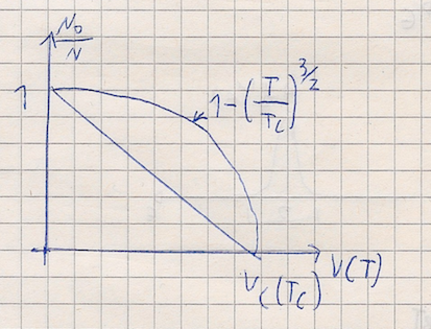
\includegraphics[width = \textwidth]{Zeichnungen/32.pdf}
  \caption{.}
  %\label{fig:Bild}
\end{figure}
\begin{align}
    \underarrow{\frac{N_0}{N}}{N_0\hat=\text{Grundzustands Besetzung}}&=
    \begin{cases}
        0 & v>v_c \\
        1-\frac{v}{v_c} \hat= 1- \left(\frac{T}{T_c}\right)^2  & (\text{für } v<v_c , T<T_c) 
    \end{cases}\\
    v_c(T) &= \frac{\lambda_T^3(T)}{\zeta\left({\frac32}\right)} \quad \lambda_T = \frac{h}{\sqrt{2\pi M \kB T}} \\
    z &= e^{\beta \mu} = 
    \begin{cases}
        1 \quad \text{für} & \frac{v}{\lambda_T^3}\leq \frac{1}{\zeta{\frac32}}\\
        \text{Lösung von } & \frac{v}{\lambda_T^3} = \frac1{g_{\frac32}(z)}
    \end{cases}
\end{align} 

%Bild33


\paragraph{Zustandsgleichung}

\begin{align}
    \frac{p}{\kB T}=\frac{1}{\lambda_T^3}g_\frac52(z) 
\end{align}

%p-T Diagramm: #caption 
%Bild34

\begin{align}
    p_c(T)&=P(v_c(T),T) \\
    &= \frac{\kB T}{\lambda_T^3} \zeta \left(\frac52 \right) = \left( \frac{M}{2 \pi \hbar^2} \right)^\frac32 \zeta \left(\frac52\right) (\kB T)^\frac52 \\
    p_c&=\text{const. für $T<T_c$ unabhängig von v}  \\
    p\leq p_c \text{für $T=$const.} \\
    \tdif{p_c}{T}&=\frac52 \left( \frac{M}{2 \pi \hbar^2} \right)^\frac32 \zeta(\frac{5}{2})(\kB T)^\frac{3}{2}=\frac52\kB \frac{\zeta\left(\frac52\right)}{\lambda_T^3}\frac{\zeta\left(\frac32 \right)T}{\zeta\left(\frac32 \right)T}\\
    & =\frac{1}{T v_c}\left[\frac{5}{2}\kB T \frac{\zeta(\frac52)}{\zeta(\frac32)}\right]=\frac{Q_L}{T \Delta v} \\
\end{align}

Form einer Clausius--Clapeyron-Gleichung
\begin{align}
    & \tdif{p_L}{T}=\frac{S_1-S_2}{v_1-v_2}=\frac{Q_L}{T \Delta v} \qquad \text{(z.B. Wasser/Eis)}\\
    \Rightarrow \text{Latente Wärme}\\
    & Q_L=\frac52 \kB T \frac{\zeta\left(\frac52\right)}{\zeta\left(\frac32\right)}
    \intertext{Annahmen}
    v(\text{Grundzustand})&=0\\
    v(\text{Rest})&=v_c \\
    \intertext{Zwei-Phasen-Modell:} 
    \intertext{\quad \quad 1. Phase: Grundzustandskondensat} 
    \intertext{\quad \quad 2. Phase: Rest aller Anregung $\epsilon>\epsilon_0=0$} 
    \intertext{$T<T_c$ Koexistenz beider Phasen} \\
\end{align}
\paragraph{Duhen-Gibbs Relation:} 
\begin{align}
    U&+pV- \mu N -TS =0 \\
    \frac{S}{N\kB}&=\frac{\beta}{N}\left[U+\frac32U-\mu N\right] \\
    &= \frac52 \beta\left(\frac{U}{N}\right)-\beta\mu \ln z \\
    &= \frac52 \frac{v}{\lambda^3_T}g_\frac{5}{2}(z)-\ln z \\
    \frac{S}{N\kB}&=
    \begin{cases}
        \frac52\frac{v}{\lambda^3_T}g_\frac52(z)-\ln z & T>T_c\\
        \frac52\frac{v}{\lambda^3_T}\zeta\left(\frac52\right)  & T<T_c
    \end{cases}
\intertext{Entropie ist an $T_c$ stetig}
    \frac{C_v}{\kB v}=\frac{1}{v\kB}\pdif{U}{T}[N,V]&=\frac52 \frac32 \frac{1}{\lambda_T^3} g_\frac{5}{2}(z)+ \frac{3}{2} \frac{T}{\lambda_T^3}g'_\frac{5}{2}(z)\pdif{z}{T}\biggr\vert_{N,v}\\
    U &= \frac32 \kB T \frac{V}{\lambda_T^3} g_\frac52 (z) \\
    \Aboxed{g'_U(z)&=\frac{1}{z}g_{n-1}(z)} \\
    g_\frac32 (z) &= \frac{\lambda_T^3}{v} \biggr\vert \pdif{}{T}[N,V] \quad \quad (N=...)^{T>T_c}\\
    g'_{\frac32}(z) \pdif{z}{T}[N,V] &= -\frac32 \frac{\lambda_T^3}{v T}\\
    \Rightarrow \pdif{z}{T}[N,V] &= -\frac32 \frac{\lambda_T^3}{v T}\frac{z}{g_\frac12(z)} \quad \quad \frac{1}{v}=\frac{N}{V} \\
    \frac{C_V}{\kB V} &= \frac{15}{4} \frac 1\lambda_T^3 g_\frac52(z) - \frac94 \frac{\cancel{T}}{\cancel{\lambda_T^3}} \frac{g_\frac32}{\cancel{Z}} \frac{\cancel{\lambda_T^3}}{\cancel{v T}} \frac{\cancel{Z}}{g_\frac12(z)} \qquad \biggr\vert \cdot \frac VN\\
    \Aboxed{\frac{C_V}{\kB N} &= \frac{15}{4} \underbrace{\frac{v}{\lambda_T^3}}_{\frac1{g_\frac52(z)} g_\frac52(z) - \frac94 \frac{g_\frac32(z)}{g_\frac12(z)}}}\\
    \lim_{z \to 1^-} \frac{1}{g_\frac12}(z) &= 0\\
    \frac{C_V}{N} \text{ist stetig an $T_C$}\\
    \frac{C_V}{\kB N}&=
    \begin{cases}
        \frac{15}{4} \frac{v}{\lambda_T^3}g_\frac52(z)-\frac94 \frac{g_\frac32(z)}{g_\frac12(z)} &T>T_c\\
        \frac{15}{4} \frac{v}{\lambda_T^3} \zeta\left(\frac52 \right)\propto T^{\frac32} & T\leq T_c
    \end{cases}
\end{align} 
%Bild35
Ehrenfest: Phasenübergang 3.Ordnung \\

Bose-Einstein-Kondensation 
\begin{enumerate}
    \item Phasenübergang 1.Ordnung in zwei Phasen(Fluid ) Moden
    \item Phasenübergang 3.Ordnung für das Gesamtsystem
\end{enumerate}